\documentclass{article}

\usepackage[utf8]{inputenc}
\usepackage[spanish,es-tabla]{babel}
\usepackage{babelbib}
\usepackage{geometry}
\usepackage{mathtools}
\usepackage{graphicx}
\usepackage{float}
\usepackage{multicol}

\geometry{letterpaper,tmargin=2cm,bmargin=2cm,lmargin=2cm,rmargin=2cm}

\begin{document}

\begin{titlepage}
    \centering
    \vspace{2cm}

    {\huge\bfseries Análisis de un sistema no lineal para el tratamiento del VIH\par}
    \vspace{5cm}
    {\Large\itshape Alejandro Salgado Gómez\par}
    \vfill

    Profesor\par
    {\large Santiago Lopez Restrepo\par}

    \vfill

    {\large Modelación y simulación IV \par}
    \vspace{0.2cm}
    {\large Ingeniería Matemática \par}
    \vspace{0.2cm}
    {\large Departamento de ciencias matemáticas \par}
    \vspace{0.2cm}
    {\large Escuela de ciencias \par}
    \vspace{0.2cm}
    {\large Universidad EAFIT \par}

    \vfill

    {\large Noviembre 22 de 2017}
\end{titlepage}


\section{Planteamiento del problema}

Las estrategias para contrarrestar el VIH utilizando métodos de control están
recibiendo cada vez más atención. Estudios detallados que combinan
técnicas de modelado con resultados clínicos muestran que la fase inicial de la
infección puede ser representada utilizando modelos no lineales simples.\cite{paper}
Este hecho impulsó la producción de artículos donde se trabaja con los principios
de control con el fin de estudiar diversas estrategias para implementar terapias de dicha
enfermedad.\\

En \cite{model} se encontró un modelo no lineal con tres variables de estado, en el
cual la dinámica de una de sus variables puede ser calculada por medio de una
ecuación algebráica al asumir su cambio como instantáneo en reacción a las variaciones
de otra variable, reduciendo así el modelo a uno de dos estados.

Este modelo asume la complejidad no lineal para representar de una manera
mas acertada el efecto que las drogas usadas en el tratamiento de esta
enfermedad tienen en los pacientes, con el fin de buscar alternativas para
implementar estrategias de control en las terapias del VIH.\\

El problema que se desea abordar en este trabajo es el análisis en distintos niveles
de dicho modelo, con el objetivo de entender más a fondo su estructura y
funcionamiento, desde los detalles más generales hasta los más específicos.

\section{Objetivo general}

Analizar el sistema no lineal de ecuaciones diferenciales escogido, sus componentes y
como reacciona al cambiar sus condiciones con el propósito de aplicar la teoría
estudiada en clase.

\section{Objetivos específicos}

\begin{itemize}
    \item Reconocer parámetros, entradas y salidas del sistema escogido.
    \item Simular el sistema.
    \item Estudiar el acoplamiento de ecuaciones.
    \item Realizar un análisis completo de las gráficas.
    \item Análizar el sistema al variar entradas y condiciones iniciales.
    \item Hallar los puntos de equilibrio del sistema.
    \item Linealizar el sistema y hacer un análisis de estabilidad en los puntos de equilibrio.
\end{itemize}

\section{Antecedentes del modelo escogido}

Existen varios antecentes directamente relaciónados con el trabajo realizado en el
artículo, como lo son \cite{ieee1}, \cite{ieee2}, \cite{ieee3}. Sin embargo,
debido a la dificultad de conseguir dichos trabajos, se proponen como
antecedentes los siguientes modelos generales.

\newpage

    \subsection{Modelo SIR}

        \Large
        $$\dot{s} = -b s(t) i(t)$$
        $$\dot{i} = b s(t) i(t) - k i(t)$$
        $$\dot{r} = k i(t)$$
        \normalsize

        \vspace{0.5cm}

        \begin{table}[H]
        \begin{tabular}[t]{|p{4cm} p{3.5cm}|p{4cm} p{4cm}|}
            \hline
            \textbf{Variables de estado} & \textbf{Unidades} & \textbf{Parámetros} & \textbf{Unidades} \\
            \hline
            $s$: Población susceptible & Número de individuos & $b$: tasa de infección    & $1/(individuos * tiempo)$\\
            $i$: Población infectada   & Número de individuos & $k$: tasa de recuperación & $1/tiempo$\\
            $r$: Población recuperada  & Número de individuos &  & \\
            \hline
        \end{tabular}
        \caption{Información modelo SIR \cite{sir}}
        \label{table:sir}
        \end{table}

        \vspace{0.5cm}

        En este modelo se busca plasmar la dinámica de tres poblaciones de
        individuos, los susceptibles, quienes todavía no han sido contagiados
        por el tipo de infección a modelar, los infectados y los recuperados,
        quienes ya son inmunes.\\

        La primera ecuación muestra el cambio en la población de
        susceptibles debido al contagio que producen los infectados, la
        segunda muestra como la población de los infectados varía
        dependiendo de la cantidad de contagiados y el número de recuperados, y
        por último en la tercera, se determina como es el proceso de cura
        de los individuos infectados.

    \subsection{Modelo predador-presa}

        \Large
        $$\dot{p} = \alpha p(t) - \beta p(t) d(t)$$
        $$\dot{d} = \lambda p(t) d(t) - \gamma d(t)$$
        \normalsize

        \vspace{0.5cm}

        \begin{table}[H]
        \begin{tabular}[t]{|p{4cm} p{3.5cm}|p{4.5cm} p{4cm}|}
            \hline
            \textbf{Variables de estado} & \textbf{Unidades} & \textbf{Parámetro} & \textbf{Unidades} \\
            \hline
            $p$: Población presas       & Número de individuos & $\alpha$: tasa nacimiento presas    & $1/tiempo$\\
            $d$: Población depredadores & Número de individuos & $\beta$: tasa caza                  & $1/(individuos * tiempo)$\\
                                        &                      & $\lambda$: tasa alimentación        & $1/(individuos * tiempo)$\\
                                        &                      & $\gamma$:  tasa muerte depredadores & $1/tiempo$\\
            \hline
        \end{tabular}
        \caption{Información modelo predador-presa \cite{predator}}
        \label{table:predator}
        \end{table}

        \vspace{0.5cm}

        En este modelo se tienen dos poblaciones, presas y depredadores, los
        cuales presentan un comportamiento de crecimiento exponencial en
        ausencia del otro (positivo para las presas y negativo para los
        predadores). En este modelo la primera ecuación muestra como el
        crecimiento exponencial de las presas es diezmado por la acción de los
        depredadores y la segunda ecuación define como la cantidad de presas
        removidas influye en el decrecimiento de la población de depredadores.

\newpage

\section{Modelo escogido}

    \Large
    \begin{equation}
    \dot{x_1} = s -dx_1 - (1-u_1) \beta x_1 x_3
    \end{equation}
    \begin{equation}
    \dot{x_2} = (1-u_1) \beta x_1 x_3 - \mu x_2
    \end{equation}
    \begin{equation} \label{eq:3}
    \dot{x_3} = (1-u_2) k x_2 - c x_3
    \end{equation}
    \normalsize

\vspace{1cm}

    \begin{table}[H]
    \centering
    \begin{tabular}{|p{6cm} p{2.5cm}|}
        \hline
        \textbf{Variables de estado} & \textbf{Unidades} \\
        \hline
        $x_1$: Concentración de células saludables & $celulas / mm^3$\\
        $x_2$: Concentración de células infectadas & $celulas / mm^3$\\
        $x_3$: Concentración de virus libre        & $copias / mm^3$\\
        \hline
    \end{tabular}

    \vspace{0.5cm}

    \begin{tabular}{|p{8cm} p{2.5cm}|}
        \hline
        \textbf{Entradas} & \textbf{Unidades} \\
        \hline
        $u_1$: Eficiencia para prevenir la infección              & Adimensional \\
        $u_2$: Eficiencia para evitar la creacion de virus libres & Adimensional \\
        \hline
    \end{tabular}

    \vspace{0.5cm}

    \begin{tabular}{|p{7cm} p{2cm} c|}
        \hline
        \textbf{Parámetro} & \textbf{Valor} & \textbf{Unidades} \\
        \hline
        $d$: Tasa de muerte natural de las células      & 0.02            & $s^{-1}$\\
        $k$: Tasa de producción de virus libres         & 100             & $s^{-1}$\\
        $s$: Tasa de producción de células sanas        & 10              & $mm^{-3} s^{-1}$\\
        $\beta$: Tasa de infección                      & $2.4 * 10^{-5}$ & $mm^3 s^{-1}$\\
        $\mu$: Tasa de muerte de las células infectadas & 0.24            & $s^{-1}$\\
        $c$: Tasa de muerte de los virus libres         & 2.4             & $s^{-1}$\\
        \hline
    \end{tabular}
    \caption{Información del modelo escogido completo \cite{model}}
    \label{table:modelComplete}
    \end{table}

\vspace{0.5cm}

En este modelo se busca plasmar la dinámica del virus VIH con el uso de tres
variables de estado que representan las células saludables, las infectadas y la
concentración de células libres en el cuerpo.\\

En la primera ecuación se muestra la dinámica de las células sanas y como su
disminución se ve afectada tanto por su muerte natural como por la influencia
del virus, en la segunda se expresa el cambio en las células
contaminadas como el contagio de células sanas menos una tasa de muerte natural
de células infectadas y por último en la tercera, se plasma el proceso
por el cual las células contaminadas liberan más virus en el sistema, los
cuales a su vez también tienen una tasa de muerte natural que los disminuye.\\

\newpage

    \subsection{Modelo reducido}

    \Large
    $$\dot{x_1} = s -dx_1 - (1-u) \frac{\beta k}{c} x_1 x_2$$
    $$\dot{x_2} = (1-u) \frac{\beta k}{c} x_1 x_2 - \mu x_2$$
    \normalsize

    \vspace{0.5cm}

    \begin{table}[H]
    \centering
    \begin{tabular}{|p{6cm} p{2.5cm}|}
        \hline
        \textbf{Variables de estado} & \textbf{Unidades} \\
        \hline
        $x_1$: Concentración de células saludables & $celulas / mm^3$\\
        $x_2$: Concentración de células infectadas & $celulas / mm^3$\\
        \hline
    \end{tabular}

    \vspace{0.5cm}

    \begin{tabular}{|p{8.5cm} p{2.5cm}|}
        \hline
        \textbf{Entradas} & \textbf{Unidades} \\
        \hline
        $u$: esta entrada es usada para simplificar las ecuaciones del modelo,
             tiene un valor de $u_1+u_2-u_1 u_2$ & Adimensional \\
        \hline
    \end{tabular}

    \vspace{0.5cm}

    \begin{tabular}{|p{7cm} p{2cm} c|}
        \hline
        \textbf{Parámetro} & \textbf{Valor} & \textbf{Unidades} \\
        \hline
        $d$: tasa de muerte natural de las células      & 0.02            & $s^{-1}$\\
        $k$: tasa de producción de virus libres         & 100             & $s^{-1}$\\
        $s$: tasa de producción de células sanas        & 10              & $mm^{-3} s^{-1}$\\
        $\beta$: tasa de infección                      & $2.4 * 10^{-5}$ & $mm^3 s^{-1}$\\
        $\mu$: tasa de muerte de las células infectadas & 0.24            & $s^{-1}$\\
        $c$: tasa de muerte de los virus libres         & 2.4             & $s^{-1}$\\
        \hline
    \end{tabular}
    \caption{Información modelo escogido reducido \cite{model}}
    \label{table:modelReduced}
    \end{table}

    \vspace{0.5cm}

Este modelo es bastante similar al anterior, tanto en estructura como en
aplicación, se puede ver basicamente como su simplifación. Los cambios
realizados son, en primer lugar, la eliminación de $x_3$ como variable de
estado al encontrar que su cambio respecto a las variaciones de $x_2$ sucede de
manera casi instantánea, lo que permite prescindir de $x_3$ como variable de
estado al expresarla como una ecuación algebráica, reduciendo así el modelo a
segundo orden.  Y en segundo lugar, la combinación de $u_1$ y $u_2$ para formar una
nueva entrada, con el objetivo simplificar las ecuaciones y facilitar el
entendimiento del modelo.

\section{Análisis de las ecuaciones}

En esta sección se discutirá con mas detalle la estructura del modelo escogido
en su versión reducida, ya que es esta la que se usará para el resto del trabajo,
debido a que representa el sistema que se desea estudiar de una manera más simple.

    \subsection{Proceso de reducción}

    El modelo pudo ser reducido al observar la relación que existe
    entre las variables $x_2$ y $x_3$, donde después de un periodo corto de
    tiempo se vuelven proporcionales, tal como se muestra en la Figura \ref{fig:relacion}.

    Ahora, en (\ref{eq:3}) puede ser vista como un sistema lineal estable con
    $x_2$ como entrada, en donde la estabilidad se alcanza rápidamente, por lo
    que al hacer $\dot{x_3} = 0$ se obtiene

    \Large
    $$x_3 = (1-u_2) \frac{k}{c} x_2$$
    \normalsize

    Y luego de reemplazar esta expresión en las otras dos ecuaciones se obtiene el
    modelo reducido con una entrada $u = u_1 + u_2 - u_1 u_2$.

    \begin{figure}[h!]
        \centering
        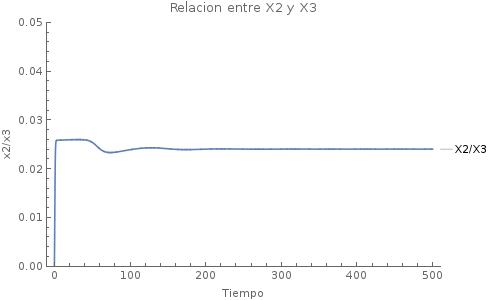
\includegraphics[scale=0.5]{Images/Vih-x2-x3}
        \caption{Relación entre las variables $x_2$ y $x_3$.}
        \label{fig:relacion}
    \end{figure}

    \newpage

    \subsection{Suposiciones e información general del modelo}

    El modelo tiene pocas suposiciones, la principal de ellas es tomar todos
    párametros como constantes, tal como la tasa de producción y muerte de las
    células sanas e infectadas, o las tasas de produccion y muerte de virus libres.

    Además de esto, el modelo plantea que no es posible eliminar la infección
    por completo, característica que se esperaría en un caso real de la
    enfermad.\\

    Es importante mencionar que el modelo se puede trabajar tanto para
    individuos infectados como para aquellos que se ecuentran sanos, esto dependiendo
    de si el valor de la variable $x_2$ es distinta de cero o no, respectivamente.
    Aunque se espera que sea utilizado en situaciones de infección, ya que de lo
    contrario las dinámicas que se generan no son tan interesantes.\\

    Ahora, de entre la información general del modelo se puede destacar
    la similitud con los modelos propuestos como antecedentes, específicamente
    en aspectos como la reducción de las poblaciones debido a la infección, su
    contagio y la muerte de los virus, tal como en el modelo SIR, y en la
    decaída de la poblaciones por una tasa de muerte, donde se puede ver cierta
    similitud con el modelo predador-presa.

    En segundo lugar es importante resaltar como las tasas de infección de las
    células sanas y la tasa de creación de virus libres pueden ser
    influenciadas con el efecto de drogas que afecten el desarrollo del virus.
    Dicha influencia se modela con las variables de entrada, donde $u_1$
    toma valores entre 0 y 1, representando la eficiencia de drogas ITR
    (Inhibidores de la Transcriptasa Inversa) que pueden reducir la propagación
    del virus. Y la variable $u_2$, que toma valores en el mismo intervalo, y
    representa la acción de drogas PI (Inhibidores de proteasa), las cuales
    previenen que las células infectadas produzcan más virus libres,
    permitiendo así ejercer un control sobre el desarrollo del virus en el
    cuerpo. Cabe resaltar también, que en la actualidad ninguna droga llega a una
    eficiencia del 100\% por lo cual un valor cercano a 1 en las entradas que
    representan su efecto ocasiona que la simulación tome una condición cada vez
    más teórica.\cite{model}\\

    Finalmente, aunque aun no es tratado de manera detallada en este trabajo,
    existen otros modelos relacionados como el presentado en \cite{ieee4},
    los cuales en las secciones de control tienen suposiciones de linealidad en
    algunas de las variables que manipulan, mientras que en este modelo la
    dependencia del control no es lineal, lo que conlleva a un trabajo de álgebra
    mas complicado, pero permite representar de una manera mas acertada la
    situación que se desea modelar.\\

    \subsection{Acoplamiento de ecuaciones y parámetros}

    Tal como se mencionó anteriormente, la descripción del modelo reducido es
    similar a la que se dio del modelo original en una sección anterior, sin
    embargo, en esta parte se describirán con mas detalle los componentes de las
    ecuaciones que describen el comportamiento del sistema con mas detalle.\\

    En primer lugar se tiene la ecuación que representa el cambio de la
    concentración de células sanas, en esta ecuación se tienen tres términos,
    el primero es la producción de células sanas que tiene la persona, a las
    cuales se les resta el segundo término, que representa la cantidad de
    células que mueren por causas naturales. Finalmente, se tiene la parte de la
    ecuación que da información sobre la tasa de infección, esta tasa es
    proporcional al producto de $x_1$ y $x_3$, pero debido a la reducción del
    modelo queda expresado como una relación entre $x_1$ y $x_2$, donde se
    tiene un factor que relaciona la tasa de producción y muerte de células
    libres con el resto del término, y de manera análoga al primer modelo se
    tiene otro factor que integra los efectos de medicamentos en el desarrollo
    del virus.

    En segundo lugar se tiene la ecuación que representa el cambio en la concentración
    de células infectadas, proceso que esta expresado como la diferencia entre el
    último término de la primera ecuación, el cual representa su crecimiento, y
    la cantidad de células infectadas que mueren.

    Finalmente, se puede observar claramente el acoplamiento entre las ecuaciones
    debido a la utilización del mismo término tanto para calcular la reducción de las
    células sanas en la primera ecuación, como el crecimiento del número
    de céluas infectadas en la segunda, generando así una fuerte dependencia entre
    las dos ecuaciones.

\section{Diagrama de estados}

\begin{figure}[h!]
    \centering
    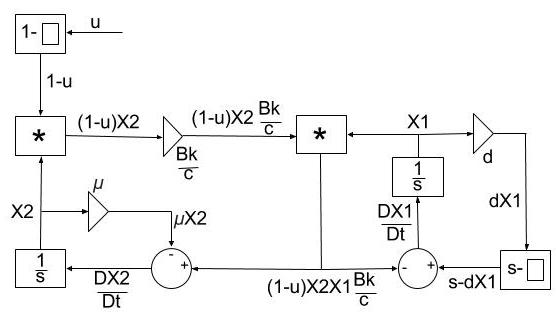
\includegraphics[width=\textwidth]{Images/State-diagram.jpeg}
    \caption{Diagrama de estados.}
    \label{fig:state-diagram}
\end{figure}

En este diagrama $s -$ y $1-$ representan las operaciones de sumar el negativo
de su entrada al valor de $s$ y $1$ respectivamente, $*$ representa la
multiplicación de dos entradas y $\frac{1}{s}$ representa un integrador.

\section{Simulaciones}

Las siguientes simulaciones fueron realizadas con la ayuda del software Mathematica
\cite{mathematica}, el código usado puede ser encontrado en
https://github.com/AlejandroSalgadoG/Miscellaneous/tree/master/Mathematica/Vih.

\begin{itemize}
    \item Modelo con entrada constante.
    \item Modelo con variación en las entradas.
    \item Modelo con diferentes condiciones iniciales.
    \item Trayectorias de estado con condiciones iniciales aleatorias.
\end{itemize}

Los valores que se utilizaron en cada simulación se presentan en el lado
izquierdo de las imágenes. los primeros dos valores corresponden a las
condiciones iniciales de $x_1$ y $x_2$ respectivamente, el siguiente valor
corresponde a la entrada, y finalmente el tercer campo da información sobre el
tiempo en el cual la entrada sufre la modificación especificada en el último
campo de la ventana. Es importante mencionar que este último campo corresponde al valor
total de la entrada, no a una desviación.

\begin{figure}[H]
    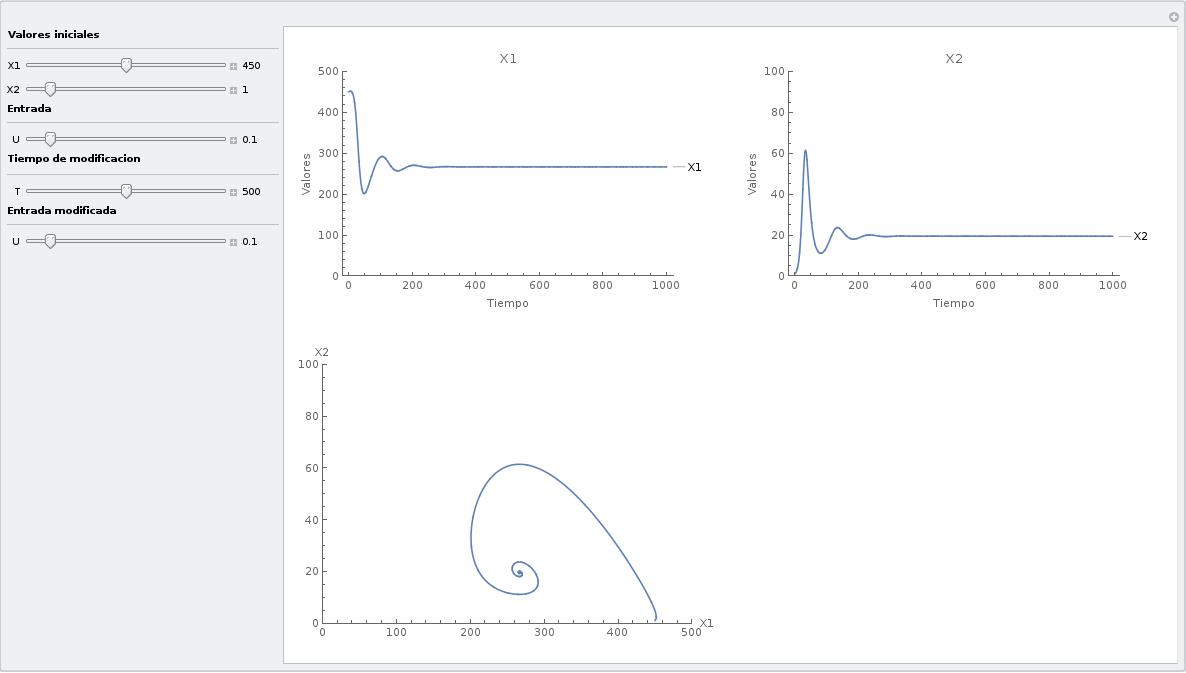
\includegraphics[width=\textwidth]{Images/Vih-u-constante}
    \caption{Simulación con entradas constantes.}
\end{figure}

En esta simulación se muestra el comportamiento del sistema con entrada constante,
tal como se puede ver en las gráficas el sistema presenta una oscilación inicial
que representa el crecimiento de las células infectadas y el decremento de las
células sanas hasta llegar a un punto de equilibrio donde las dos poblaciones se
estabilizan.

\begin{figure}[H]
    \centering
    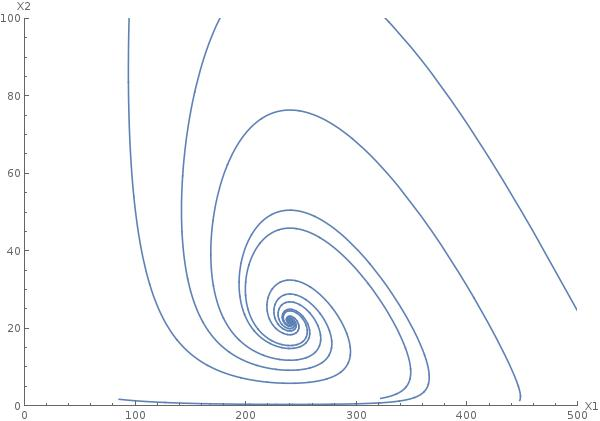
\includegraphics[scale=0.4]{Images/Vih-random}
    \caption{Trayectorias de estado con condiciones iniciales aleatorias.}
\end{figure}

En este diagrama se muestran varias trayectorias de estado desde distintas
condiciones iniciales, con la entrada constante, a partir de esta gráfica se
puede observar como el sistema tiende a presentar un comportamiento oscilante al
inicio de las simulaciones, representado en los giros que se dan el plano,
las cuales van disminuyendo hasta converger a un punto estable.

\begin{figure}[H]
    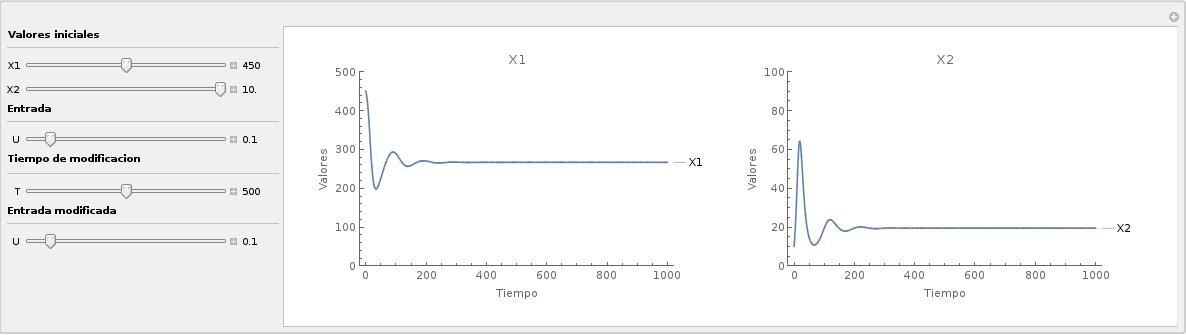
\includegraphics[width=\textwidth]{Images/Vih-more-infected.jpeg}
    \caption{Simulación con un incremento en la cantidad de células infectadas iniciales.}
\end{figure}

Basado en lo mostrado en esta simulación se puede ver como al incrementar el
número de células infectadas que el modelo tiene inicialmente, los picos de
las variables de estado se generan un poco más rapido, lo cual se puede interpretar como una
reacción mas acelerada de crecimiento de en las células infectadas y un
decrecimiento en las células sanas.

\begin{figure}[H]
    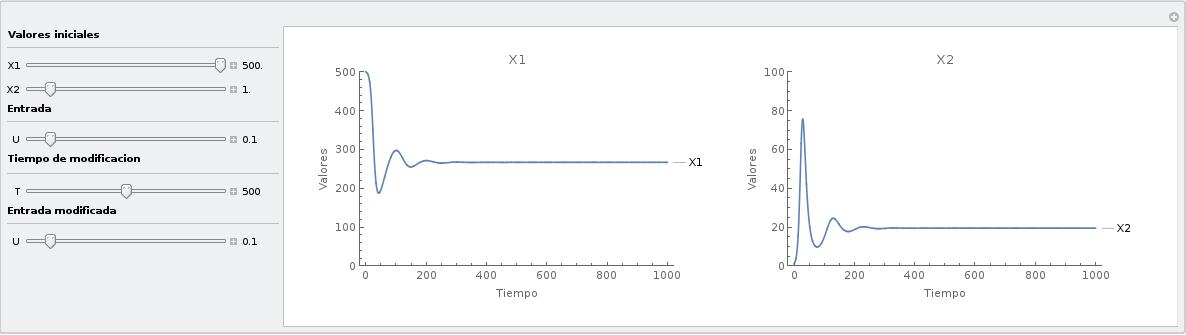
\includegraphics[width=\textwidth]{Images/Vih-more-healthy.jpeg}
    \caption{Simulación con un incremento en la cantidad de células sanas iniciales.}
\end{figure}

Se puede observar que en el caso de aumentar el número de células sanas, se obtienen
picos mas elevados al inicio de la simulación, lo cual se puede interpretar como
una reacción mas agresiva en cuanto al cambio el número tanto de las células infectadas
como de las sanas.

\begin{figure}[H]
    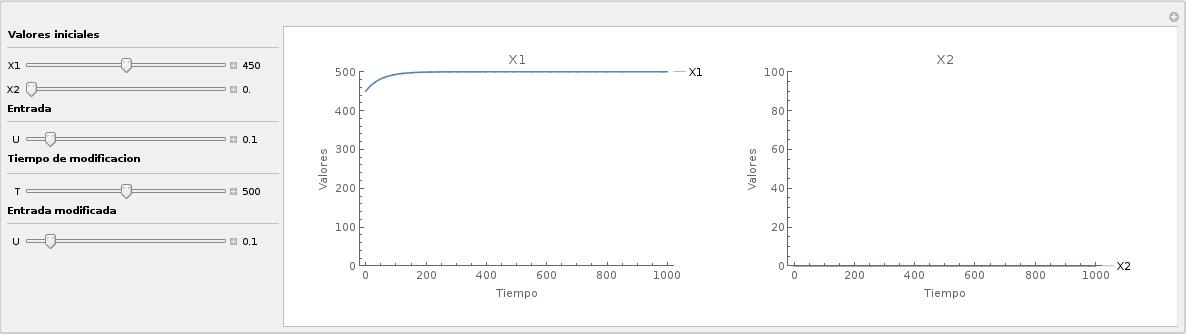
\includegraphics[width=\textwidth]{Images/Vih-healthy.jpeg}
    \caption{Simulación de una persona sana.}
\end{figure}

Tal como es de esperarse, en el caso de que la persona no este infectada las células
sanas pueden reproducirse sin problemas, siendo capaces de aumentar su número hasta
estabilizarse, mientras que la población de células infectadas se mantiene
en cero.

\begin{figure}[H]
    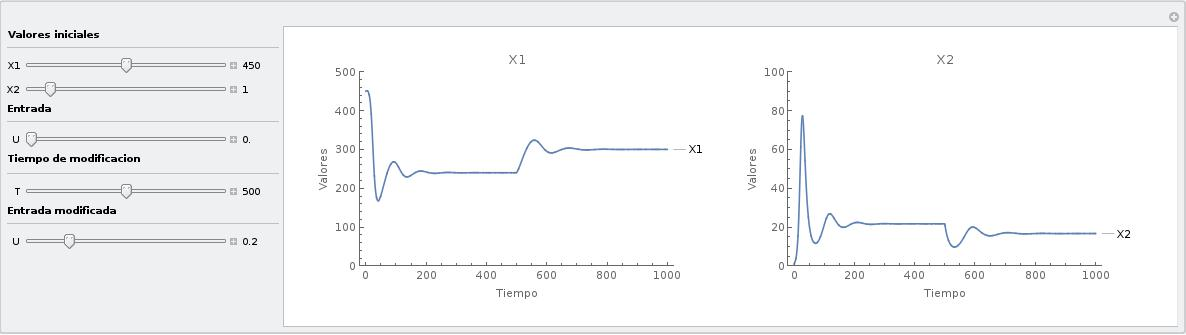
\includegraphics[width=\textwidth]{Images/Vih-noinput-input.jpeg}
    \caption{Simulación con entrada nula que se incrementa.}
\end{figure}

Las siguientes simulaciones tienen el objetivo de ver el comportamiento del
sistema al variar su entrada. En este caso se tiene una simulación en la que
el paciente no recibe medicamentos en un inicio, pero luego de un tiempo se comienza
a suministrar una dosis. El resultado de esta variación es una oscilación en ambas
poblaciones de células que converge en un incremento en el número
de las células sanas y un decremento leve en el número de las infectadas.

\begin{figure}[H]
    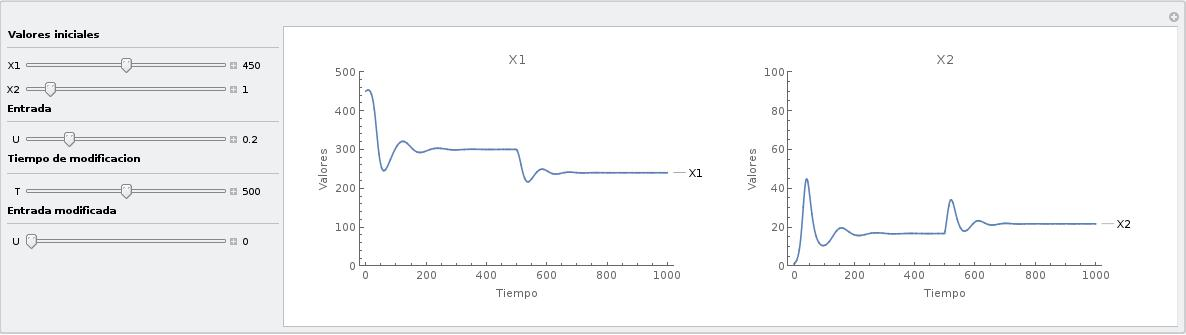
\includegraphics[width=\textwidth]{Images/Vih-input-noinput.jpeg}
    \caption{Simulación con decremento en la entrada.}
\end{figure}

En este caso se observa una simulación en la que la persona analizada recibe
medicamentos en un principio pero luego se dejan de suministrar. Como es de esperarse
luego de una característica oscilación el número de células sanas se disminuye
y el número de células infectadas se incrementa.

\begin{figure}[H]
    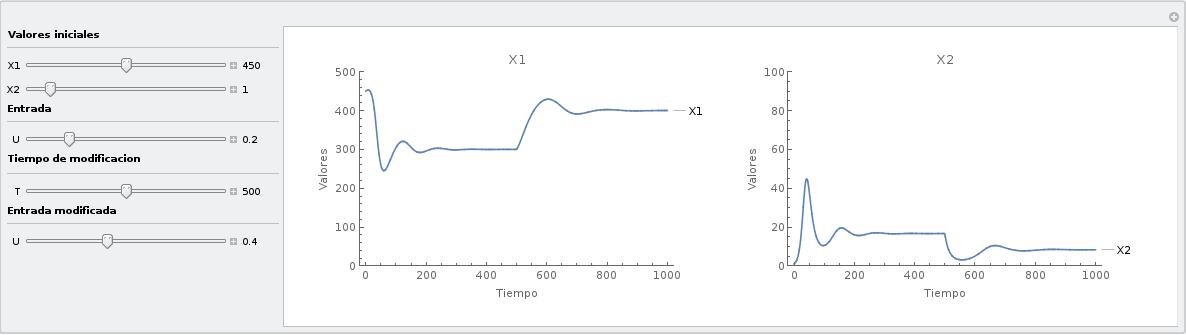
\includegraphics[width=\textwidth]{Images/Vih-input-moreinput.jpeg}
    \caption{Simulación con incremento en la entrada.}
\end{figure}

Por último, en esta simulación se puede observar el caso en el que se
suministran medicamentos desde el principio y luego de un tiempo se incrementa
la dosis, los resultados muestran que, de nuevo, en un principio el sistema se
estabiliza hasta que llega el nuevo valor de la entrada, la cual
tiene, después de su oscilación, el efecto de aumentar el número de
células sanas que son producidas y diezma el número de las células infectadas
en el sistema.

\section{Linealización}

En esta sección se discutir la linealización del modelo, es importante aclarar
que a partir de este punto todas las simulaciones fueron realizadas con ayuda
del software MATLAB y Simulink. En la Tabla \ref{table:linearInfo} se muestra
la información acerca de la linealización que se realizó.

\begin{table}[H]
\begin{equation*}
    \begin{cases}
       X1 = 266.677 & \text{Cantidad inicial de células sanas} \\
       X2 = 19.4406 & \text{Cantidad inicial de células infectadas}\\
       u = 0.1      & \text{Efectividad del medicamento suministrado}
    \end{cases}
\end{equation*}

\begin{multicols}{4}
    \begin{equation*}
        A = \begin{bmatrix}
                -0.0375 & -0.2400\\[0.25cm]
                0.0175 & 0.0000
            \end{bmatrix}
    \end{equation*}

    \begin{equation*}
        B = \begin{bmatrix}
                5.1844\\[0.25cm]
                -5.1844
            \end{bmatrix}
    \end{equation*}

    \begin{equation*}
        C = \begin{bmatrix}
                1 & 0\\[0.25cm]
                0 & 1
            \end{bmatrix}
    \end{equation*}

    \begin{equation*}
        D = \begin{bmatrix}
                0\\[0.25cm]
                0
            \end{bmatrix}
    \end{equation*}

\end{multicols}
\caption{Información sobre la linealización}
\label{table:linearInfo}
\end{table}

Al buscar los valores propios de la matriz $A$ se encontró que corresponden a
$-0.0187 + 0.0620i$ y $-0.0187 - 0.0620i$, los cuales corresponden a números
complejos conjugados con parte real negativa, implicando que el punto de equilibrio
escogido es del tipo espiral, el cual presenta un comportamiento asintóticamente
estable.

\subsection{Simulaciones}

Se realizaron diferentes simulaciones variando el valor de la entrada para
observar el comportamiento del sistema lineal y compararlo con su versión no
lineal. En la Figura \ref{sim:linear1} se puede observar como al incrementar la
entrada solo un poco, el sistema lineal sigue representado de manera casi
perfecta el comportamiento de su contraparte no lineal, sin embargo, tal como
se puede ver en la Figura \ref{sim:linear2}, a medida que la entrada se aleja
cada vez más de su valor original, la similiridad que caracterizaba ambos
modelos empieza a disiparse cada vez más, hasta llegar a un punto donde dicha
similitud se pierde, debido a la lejania del punto de operación seleccionado,
tal como lo sugiere la Figura \ref{sim:linear3}, donde los dos
modelos exhiben un comportamiento diferente, especialmente en la
dinámica de las células infectadas.

\begin{figure}[H]
    \centering
    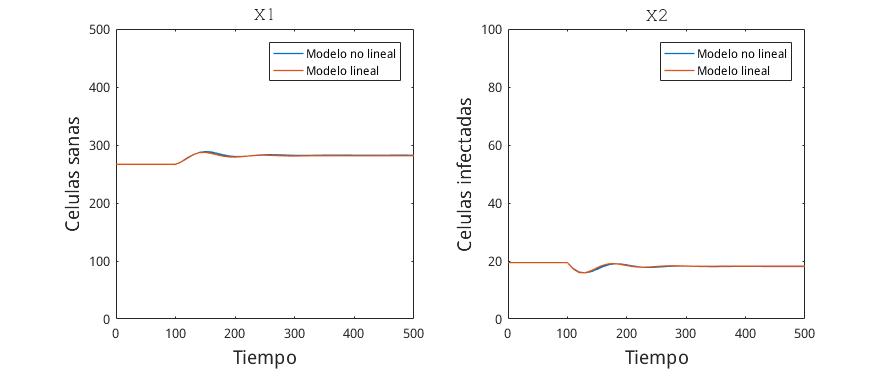
\includegraphics[scale=0.7]{Images/LinealU15.png}
    \caption{Simulación con entrada incrementada en 0.05 unidades de su valor inicial}
    \label{sim:linear1}
\end{figure}

\begin{figure}[H]
    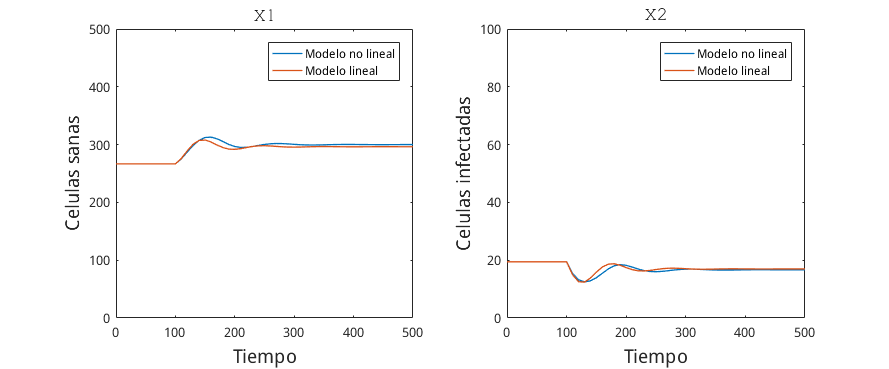
\includegraphics[width=\textwidth]{Images/LinealU20.png}
    \caption{Simulación con entrada incrementada en 0.1 unidades de su valor inicial}
    \label{sim:linear2}
\end{figure}

\begin{figure}[H]
    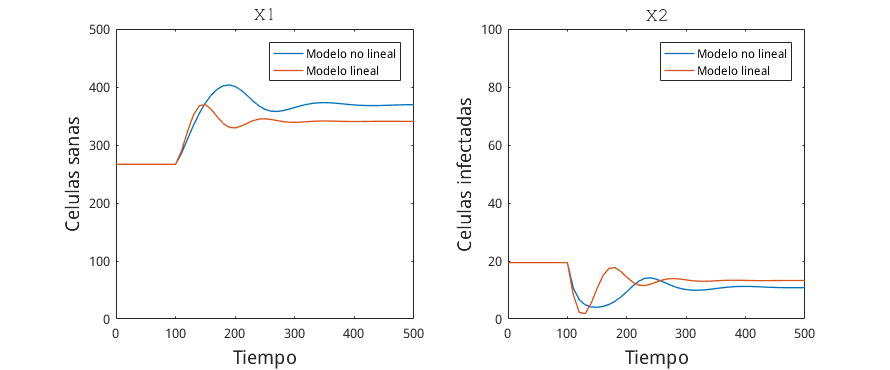
\includegraphics[width=\textwidth]{Images/LinealU35.png}
    \caption{Simulación con entrada incrementada en 0.25 unidades de su valor inicial}
    \label{sim:linear3}
\end{figure}

\section{Control}

Posteriormente se comenzó a realizar un sistema de control que permitiera
controlar la cantidad de células sanas e infectadas del modelo. Para la construcción
de dicho controlador se hizo uso del modelo lineal construido en la sección anterior,
con el objetivo de crear un control lineal por retroalimentación de
estados que puediese ser usado para este fin. El primer paso fue el cálculo de
la matriz de controlabilidad, la cual arrojó como resultado la siguiente matriz.

\begin{equation*}
    Q = \begin{bmatrix}
            5.1844  & 1.0499 \\[0.25cm]
            -5.1844 & 0.0907
        \end{bmatrix}
\end{equation*}\\

La cual resultó tener un rango igual a 2, implicando que el sistema es controlable.
Luego de conocer esta información se procedió a encontrar los valores de los polos
que permitirían controlar cada uno de las variables de estado y la ganancia necesaria
para que el controlador tuviese un comportamiento adecuado, todo esto con el objetivo de
realizar la implementación del controlador lineal sobre el modelo no lineal.
Dicho proceso se logró con el uso de las siguientes expresiones.\\

\begin{equation}\label{eq:newA}
    A' = A-BK
\end{equation}

\begin{equation}\label{eq:gain}
    G = \frac{-1}{C1 (A-BK)^{-1} * B}
\end{equation}

\subsection{Control de X1}

Para este caso se encontró que los polos $-0.4$ y $-0.2$ permiten que el
controlador manipule la cantidad de células sanas en el modelo sin presentar
sobrepicos muy pronunciados. Dichos polos fueron alcanzados al reemplazar la
matriz $A$ por una nueva matriz calculada con (\ref{eq:newA}) donde $K=[0.0566,
-0.0519]$, y de manera similar la ganacia necesaria para que el
controlador pudiese llegar a un valor de referencia establecido, fue
calculada con (\ref{eq:gain}) donde $C1 = [1, 0]$, con el objetivo de
especificar que es X1 la variable que se desea controlar, dicho proceso
arrojó como resultado una ganancia de 0.0643.\\

Se realizaron 3 simulaciones para esta variable, dos mostrando como es el
comportamiento del sistema cuando el controlador intenta aumentar la cantidad
de células sanas en el modelo y una mostrando el comportamiento en
caso de tratar de disminuir las células sanas. Es importante resaltar que este
último caso es únicamente para ilustrar el comportamiento del sistema, ya que
disminuir la cantidad de células sanas en el cuerpo empeoraría la salud de las
personas infectadas con la efermedad.\\

El primer caso que se simuló fue tratar de llevar la cantidad de células sanas
a un valor un poco mayor que el estado inicial, en la Figura \ref{fig:x1to320} se
puede observar como el controlador comienza a variar la entrada para generar el
cambio deseado en el sistema, es importante recordar que dicha entrada solo puede
tomar valores entre 0 y 1, por lo cual el cambio demora un poco más para llegar
al punto deseado que en el caso en el que no se tuviese esta restricción, además
presenta un pico alrededor del tiempo 120 debido a que la entrada
no puede tomar valores negativos, sin embargo gracias a esta
restricción el modelo se comporta de manera más realista.

\begin{figure}[H]
    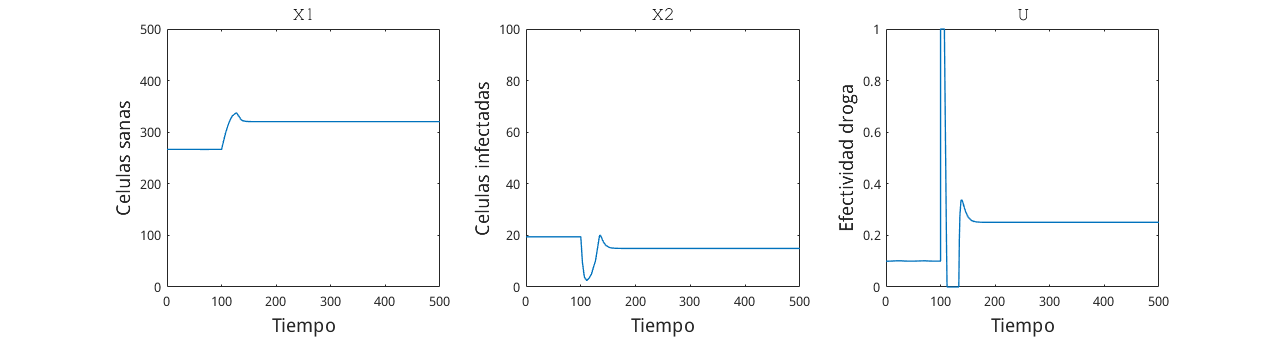
\includegraphics[width=\textwidth]{Images/ControlX1Up.png}
    \caption{Controlador tratando de llevar X1 a 320 células sanas}
    \label{fig:x1to320}
\end{figure}

En la Figura \ref{fig:x1to450} se puede observar la segunda simulación
realizada, la cual consistió en incrementar aun más el número de células sanas
en el modelo, se puede obervar como el controlador empieza a variar la entrada
para tratar de llevar el sistema al estado deseado, en este caso se hacen más
notorias las características mencionadas anteriormente, como la demora en
llegar al estado deseado o la restricción de la entrada, evidenciada en la
saturación que se presenta debido a la necesidad de seguir incrementando la
cantidad de células sanas en el cuerpo para luego suspender su uso y reducirlas
hasta llegar al punto deseado.

\begin{figure}[H]
    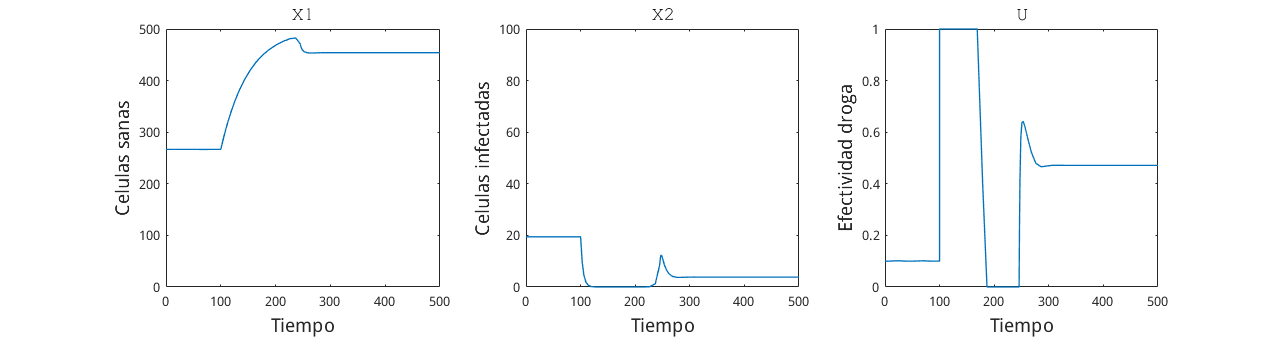
\includegraphics[width=\textwidth]{Images/ControlX1Up2.png}
    \caption{Controlador tratando de llevar X1 a 450 células sanas}
    \label{fig:x1to450}
\end{figure}

Finalmente se simuló un caso para observar el comportamiento del sistema cuando
se reduce el valor de la primera variable de estado, tal como se muestra en la
Figura \ref{fig:x1to200}, es importante mencionar que este caso busca
simplemente ilustrar el comportamiento, ya que no es aplicable en la vida real.
En este caso se encontró un comportamiento bastante particular, ya que no se
logro llegar al punto especificado como referencia, sin embargo, dicho
comportamiento puede explicarse si se considera la restricción impuesta sobre
la entrada, la cual puede tomar como mínimo un valor de 0, lo que genera que
las células sanas disminuyan por un tiempo, pero debido a las dinámicas del
sistema en ausencia de la droga suministrada, este se estabiliza antes de
llegar al punto deseado.

\begin{figure}[H]
    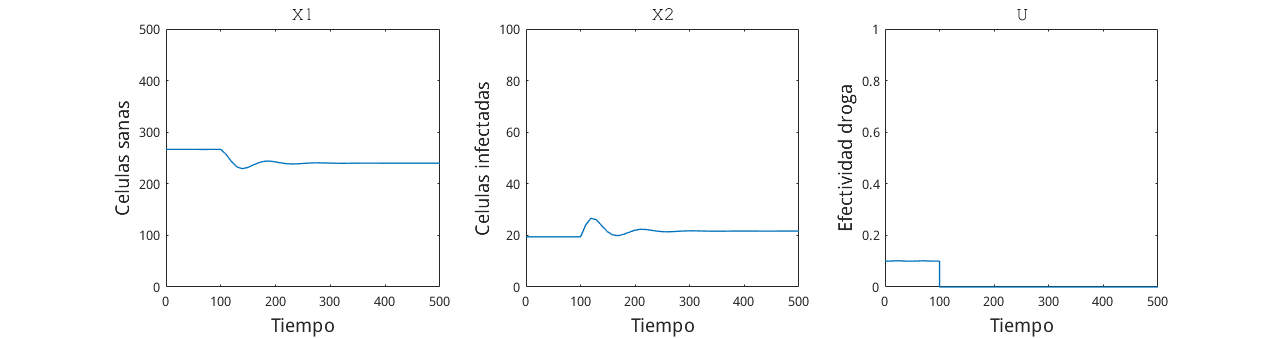
\includegraphics[width=\textwidth]{Images/ControlX1Down.png}
    \caption{Controlador tratando de llevar X1 a 200 células sanas}
    \label{fig:x1to200}
\end{figure}

\subsection{Control de X2}

Luego, en este caso se encontró que los polos $-0.1$ y $-0.05$ permiten que
el controlador manipule la cantidad de células infectadas en el modelo sin
presentar sobrepicos. De manera análoga al caso anterior, dichos polos fueron
alcanzados al reemplazar la matriz $A$ por una nueva matriz calculada con
(\ref{eq:newA}) donde $K=[-0.0013, -0.0230]$, y la ganacia
necesaria para que el controlador pudiese llegar a un valor de referencia
establecido fue calculada con (\ref{eq:gain}) donde, ahora, $C1 = [0, 1]$, con el
objetivo de especificar que es X2 la variable que se desea controlar, dicho
proceso arrojó como resultado una ganancia de -0.0482.\\

Se realizaron dos simulaciones, la primera con el objetivo de reducir la cantidad
de células infectadas en el modelo y otro caso, netamente ilustrativo, en el que
se aumentan la cantidad de estas células para observar el comportamiento del
sistema. \\

En la Figura \ref{fig:x2to13} se muestra la primera simulación, el
comportamiento es bastante normal, el controlador varía la entrada dentro del
rango permitido, es decir no hubo necesidad de saturar la entrada, para
ocacionar una disminución en la cantidad de células infectadas hasta llegar al
nivel deseado y en consecuencia se genera un aumento en la cantidad de células sanas.

\begin{figure}[H]
    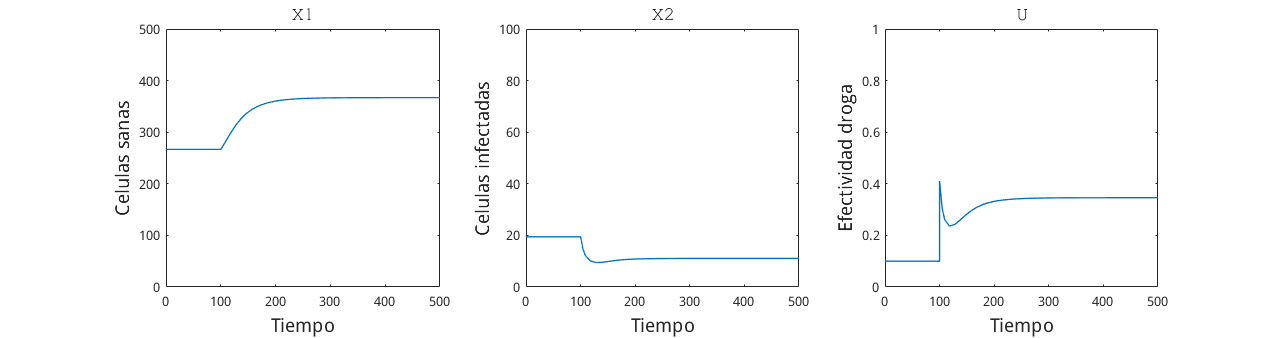
\includegraphics[width=\textwidth]{Images/ControlX2Down.png}
    \caption{Controlador tratando de llevar X2 a 13 células infectadas}
    \label{fig:x2to13}
\end{figure}

Posteriormente se simuló un caso en el que controlador tratara de aumentar
el valor de la segunda variable de estado, en este caso se encontró un resultado
bastante similar al mostrado en la Figura \ref{fig:x1to200}, ya que no se logra
llegar al valor deseado debido a la restricción de valores que la entrada puede
tomar. En esta simulación la cantidad de células infectadas se incrementa por un momento
pero luego se estabiliza en un punto defirente al deseado debido a la dinámica
propia del sistema.

\begin{figure}[H]
    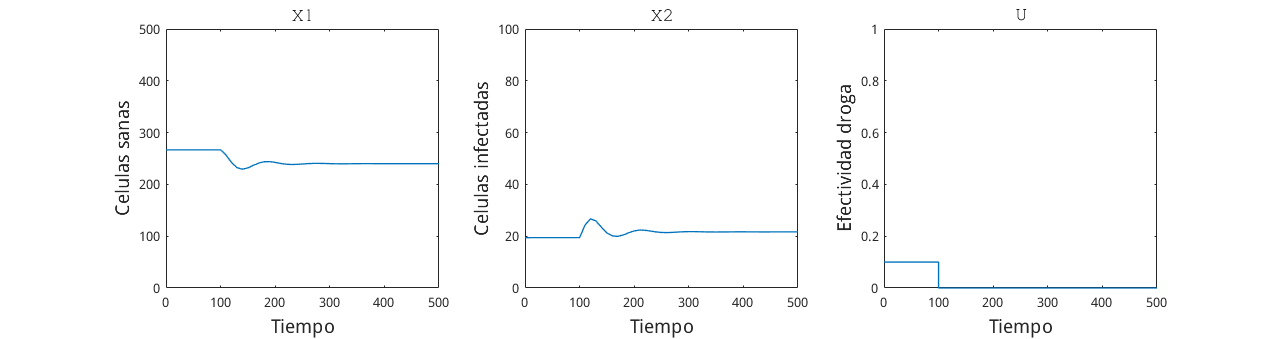
\includegraphics[width=\textwidth]{Images/ControlX2Up.png}
    \caption{Controlador tratando de llevar X2 a 30 células infectadas}
\end{figure}

\section{Estimación de parámetros}

Por último, se realizó una estimación de parámetros, el procedimiento que se realizó
fue tomar una versión del modelo no lineal con los parámetros utilizados en \cite{model}
para simular las salidas del sistema real, y se utilizó otra copia del mismo modelo
pero con los valores de los parámetros $d$, $k$ y $s$ igualados a 0 con el objetivo
de estimarlos. Las condiciones iniciales usadas corresponden a $X1 = 450$
y $X2 = 1$, con una entrada $u = 0.1$. Las simulaciones de ambos modelos pueden
ser observadas en la Figura \ref{plot:befEstimation}, donde se puede observar
un comportamiento completamente diferente en ambos modelos.\\

Luego de la estimación de parámetros se llego a un muy buen resultado, los valores
reales y los resultados obtenidos pueden ser consultados en la
Tabla \ref{table:paramInfo}, y en la Figura \ref{plot:aftEstimation} se puede
observar la nueva simulación utilizando los valores encontrados con la estimación.

\begin{figure}[H]
    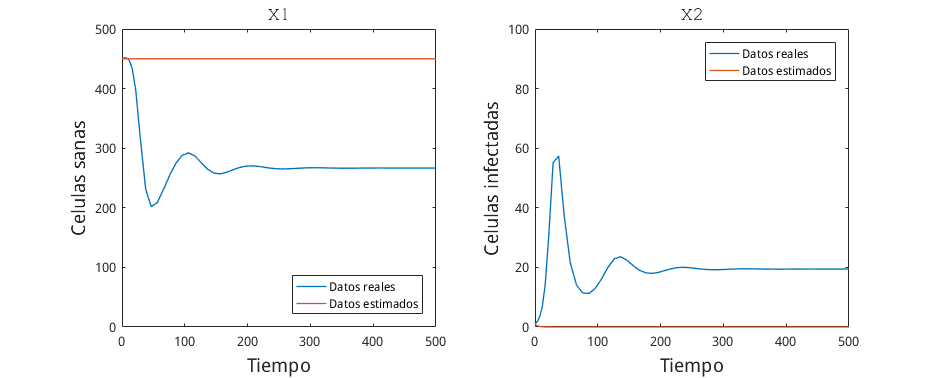
\includegraphics[width=\textwidth]{Images/BeforeEstimated.png}
    \caption{Simulación antes de la estimación de parámetros}
    \label{plot:befEstimation}
\end{figure}

\begin{table}[H]
    \centering
    \begin{tabular}{|c|c|c|}
        \hline
        Parámetro & Valor real & Valor estimado\\
        \hline
        $d$       & 0.02       & 0.02\\
        $k$       & 100        & 100.0004\\
        $s$       & 10         & 10.0119\\
        \hline
        \multicolumn{3}{|c|}{Error total (suma de cuadrados)}\\
        \hline
        \multicolumn{3}{|c|}{$3.3110$ x$10^{-07}$}\\
        \hline
    \end{tabular}
    \caption{Información sobre la estimación de parámetros}
    \label{table:paramInfo}
\end{table}

\begin{figure}[H]
    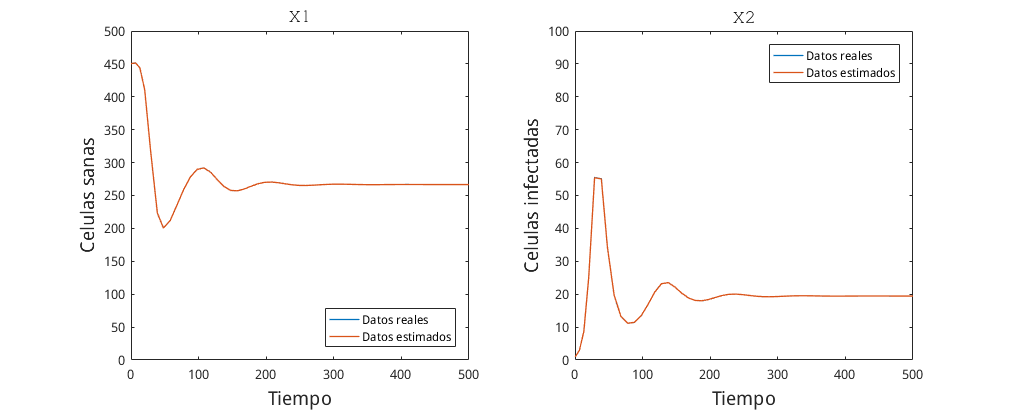
\includegraphics[width=\textwidth]{Images/Estimated.png}
    \caption{Resultados de la estimación de parámetros}
    \label{plot:aftEstimation}
\end{figure}

\section{Conclusiones}

\begin{itemize}
    \item Basado en lo ilustrado anteriormente se puede concluir que el modelo
    trabajado simula un sistema bastante estable, ya que como se pudo observar en
    las simulaciones las variables convergen tanto al cambiar la entrada como
    sus condiciones iniciales.

    \item El modelo da información acerca del desarrollo de la enfermedad
    de una manera coherente y de acuerdo a lo que se esperaría de una infección
    de VIH real, tal como se ve reflejado en el hecho de no poder curar totalmente
    a una persona, pero si reducir los efectos del virus con la ayuda de medicamentos.

    \item Se considera que la reducción del modelo fue realizada de
    una manera correcta, ayuda a lograr un entendimiento más rápido y sigue
    presentado las dinámicas de sistema de manera completa, ya que no se pierde
    información en su proceso debido a la facilidad de encontrar los valores de
    la tercera variable de estado por medio de su ecuación algebráica.

    \item Se considera que el modelo lineal encontrado fue de gran utilidad ya
    que no solo permite representar el sistema no lineal cerca del punto de
    operación, sino que permitió la implementación de un controlador para el sistema
    no lineal que funciona de una manera bastante buena.

    \item Por último, aunque se encontró que el sistema lineal construido es
    controlable, se descubrió que debido a las restricciones impuestas sobre la
    entrada al sistema y las dinámicas que rigen el comportamiento del modelo
    no es posible llevar el sistema a cualquier valor de las variables de
    estado, sin embargo aquellos casos corresponden a acciones que empeorarían
    la salud del paciente, como lo es el incremento de las células infectadas o
    el decremento de las sanas.
\end{itemize}

\bibliographystyle{unsrt}
\bibliography{Proyecto}

\end{document}
